\documentclass[]{interact}
\usepackage[outdir=./]{epstopdf}
\usepackage[natbibapa,nodoi]{apacite}
\usepackage{mathtools, fix-cm}
%\usepackage[nomarkers, nolists, tablesfirst]{endfloat}
%\renewcommand{\efloatseparator}{\mbox{}}

\title{A variation on the Chamberlin trimetric map projection}
%\author{Brenton R S Recht: brstone@gmail.com, 55 Foster St, Whitesboro, NY, 13492. ORCiD 0000-0001-7657-7218}
\date{June 2021}

\begin{document}
\maketitle
\begin{abstract}%max 250 words
   We present a variation on the Chamberlin trimetric map projection. This new
   projection, which we call the matrix trimetric projection, consists of a
   linear transformation of the squares of the distances between a given point
   and three control points. The formula of the forward projection is simpler
   than the Chamberlin projection, and admits an inverse formula which requires
   numerical iteration of only one parameter. We make comparisons between the
   two projections using a representative list of control points. The Chamberlin
   trimetric projection outperforms the matrix trimetric projection on measures
   of angle deformation and scale deformation, but the opposite is true for a
   measure of distance deformation, and the difference between the results of
   the projections is small over all measures. The forward Matrix trimetric
   projection can be calculated in half the time of the Chamberlin trimetric
   projection. We conclude that the matrix
   trimetric projection is a viable alternative to the Chamberlin trimetric
   projection, especially if an inverse is required or speed is important.

   \textit{Keywords: Chamberlin trimetric, matrix trimetric, projection,
   cartography, distortion, distance, triangulation}

\end{abstract}

\section{Introduction}
Any map projection must introduce some form of distortion. In particular, no
map projection can be both conformal (angle-preserving) and equal-area.
Projections that eliminate one form of distortion often introduce a great deal
of another form of distortion. For example, many conformal projections
drastically enlarge some areas compared to others, most notoriously the
Mercator projection, but also the stereographic and the Lambert conformal conic
projections. \citep{snyder87} A compromise map projection is one that seeks to
balance different kinds of distortion: allowing some amount of different kinds
of distortion can produce a map where none of the distortion is conspicuous.

The Chamberlin trimetric projection (CTP) is such a compromise map projection.
It is named for Wellman Chamberlin, a chief cartographer for the National
Geographic Society, which has published wall and atlas maps using his
projection. \citep{christensen} The CTP is appropriate for mapping whole
continents and large portions of continents. It may be thought of as a form of
triangulation. It can also be considered part of an ``$n$-metric'' family of
projections with the azimuthal equidistant projection and the two-point
equidistant projection, which depend on measurements from a single point and
pair of points, respectively. \citep{snyder87} Being a compromise projection,
the CTP does not perfectly preserve angle, area, or distance. Most often, the
CTP is used with the spherical approximation of the Earth: for practical
ellipsoids, distortions due to the spherical approximation are negligible
compared to distortions due to the projection itself.

The CTP is based on a simple geometric construction, using three arbitrary
control points on the sphere. However, modern computerized GISes require
algebraic formulas, which are somewhat involved for the CTP.
These formulas are presented in \citet{christensen},
and can be seen in the source code to its implementation in \citet{proj}.
In general, the length of the algorithm relates to its speed of execution.
In particular, the algorithmic form has branching logic depending on
where the given point lies with respect to the geodesics between control points,
which (as \citet{christensen} observed) can cause numerical issues.

We present a new map projection called the matrix trimetric projection
(MTP) as an alternative to the CTP. A geometric construction related to the
CTP results in a map projection that is similar but has a simpler formula. This
formula is a closed-form matrix function of the squares of the distances, and
allows for a tractable inverse. As the derivations involve matrices and linear
algebra, refer to a text such as \citet{strang80} if needed.

\section{Preliminaries}
These projections will almost always be implemented using the spherical
approximation. Formulas for that approximation are given shortly, and we'll
refer to ``the sphere'' instead of ``the ellipsoid''. In fact, the forward
formulas for the CTP and MTP are agnostic of the surface to be projected,
depending only on the result of the distance function.

We denote points on the sphere by $\mathbf v$ or subscripted versions.
$\mathbf v$ is a 3-vector with unit length lying on the unit sphere.
Using this vector form allows us to take advantage of linear algebra.
Points specified by latitude $\varphi$ and longitude $\lambda$
can be converted to a unit vector as so:\citep{kent}
\begin{equation}
\mathbf v =
\begin{bmatrix*}
  x \\ y \\ z
\end{bmatrix*}
=
\begin{bmatrix*}
 \cos(\varphi) \cos(\lambda) \\
 \cos(\varphi) \sin(\lambda) \\
 \sin(\varphi)
\end{bmatrix*}.
\end{equation}
The reverse conversion is:
\begin{equation}\begin{split}
  \varphi =& \arctan\left(\frac{z}{\sqrt{y^2 + x^2}}\right), \\
  \lambda =& \arctan\left(y, x\right),
\end{split}\end{equation}
where the 2-variable form of $\arctan$, commonly called \texttt{arctan2} or
\texttt{atan2} in numeric software libraries, is used for $\lambda$.

One statement of the distance function on the sphere is
\begin{equation}
d\left(\mathbf v_i, \mathbf v_j\right)
= R \arccos\left(\mathbf v_i \cdot \mathbf v_j\right)
\end{equation}
where $R$ is the radius of the sphere. We use a radius of 6,371 km,
approximately equal to the most common mean radii of the Earth. \citep{snyder87}
There are equivalent functions in terms of vectors
that are more numerically stable for certain range of arguments,
but this is the form we will use for derivations.

We denote points in the Euclidean plane by $\mathbf p = [x, y]$ and
subscripted versions. Planar distances are found using the usual
Euclidean norm: $\|\mathbf p_a - \mathbf p_b\|$.

Let $\mathbf v_1$, $\mathbf v_2$, $\mathbf v_3$ be control points on the
sphere, in counter-clockwise order, and let $\mathbf V$ be the matrix having
$\mathbf v_i$ as its $i$th column. Let $\mathbf p_1$ etc. be the control points
on the plane, in corresponding order, and $\mathbf P$ be the matrix having
$\mathbf p_i$ as its $i$th column. The triangles with vertices at $\mathbf v_i$
or $\mathbf p_i$ are called the control triangles: spherical or planar control
triangle, respectively, if the distinction is important. The control points
are usually chosen so that the control triangle contains or mostly contains
the geographic region of interest. For this paper,
very small triangles are excluded, as are triangles with areas of an entire
hemisphere or more: neither are typical use cases for the CTP.
Note that the planar control triangle is \textbf{not} the image of the
spherical control triangle under either projection! That image is
slightly larger, containing the planar control triangle, and has curved edges.

For both projections, $\mathbf p_i$ must be arranged such that
$d\left(\mathbf v_i, \mathbf v_j\right) = \|\mathbf p_i - \mathbf p_j\|$
for all $i$ and $j$ in $\{1, 2, 3\}$: the spherical length of the edges of the
spherical control triangle are equal to the Euclidean lengths of the planar
control triangles. Without loss of generality, also assume that
$\|\mathbf p_i\|$ is the same for all $i$, such that the circumcenter of the
control triangle lies at the origin. This assumption just removes a translation
in the plane in order to simplify the formula for the MTP: false northing and
easting can be added later. Given $\mathbf v_i$, $\mathbf p_i$ can be
constructed as follows. Let $i, j, k$ be a cyclic permutation of
$\{1, 2, 3\}$, and let $s_k = d\left(\mathbf v_i, \mathbf v_j\right)$,
such that side $k$ with length $s_k$ is opposite point $k$. The circumradius
of the Euclidean triangle with sides of length $s_k$ is \citep{isaacs}
\begin{equation}\label{eq:circumradius}
  C = \frac{\prod_i s_i}
            {\sqrt{\sum_i 2 s_i^2 s_j^2 - s_i^4}}.
\end{equation}
From the (Euclidean) law of cosines,
the interior angle $\phi_i$ at each vertex is
\begin{equation}\label{eq:phi}
  \phi_i = \arccos \left( \frac{s_k^2 + s_j^2 - s_i^2}{2 s_k s_j}\right).
\end{equation}
Then a set of points satisfying the requirements are given as so:
\begin{equation}\label{eq:planarctrlpts}
  \mathbf P = \begin{bmatrix*}[r]
  C \cos \left(2 \phi_2 \right) &
  C \cos \left(2 \phi_1 \right) &
  C \\
  C \sin \left(2 \phi_2 \right) &
  -C \sin \left(2 \phi_1 \right) &
  0 \\
\end{bmatrix*}.
\end{equation}
These points can be rotated about the origin as desired. Note that some
intermediate values in Equation \ref{eq:circumradius} may be large. This
should not cause a problem on modern computers using common geographic
units of distance, but one may wish to use a unit of measurement such
as radians of arc in these calculations and then scale the result accordingly.

\section{Forward projection}
Figure \ref{fig:chamberlin} shows the geometric construction of the CTP and
MTP. We start with the CTP. Let $\mathbf v$ denote the point to project, and
let $r_i = d(\mathbf v_i, \mathbf v)$ be the true distances from each control
point to $\mathbf v$. Figure \ref{fig:chamberlin}a shows the control triangle
on the sphere with vertices $\mathbf v_i$, the given point $\mathbf v$, and
circles of radius $r_i$ centered on $\mathbf v_i$ and passing through
$\mathbf v$. Moving to the plane, Figure \ref{fig:chamberlin}b shows circles of
the same radius $r_i$ centered on the planar control points $\mathbf p_i$. The
circles appear to all intersect at a single point, but due to the difference in
curvature between the sphere and the plane they in fact form a small triangle
with curved edges, as shown in Figure \ref{fig:chamberlin}c. In the time of
manual plotters the exact definition of this point was less important, but
\citet{christensen} and modern implementations (e.g. \citealp{proj}) use the
centroid of the small triangle, denoted $\mathbf p_c$.
Note that each pair of circles intersects in (at most) two points,
so the algorithm must choose which point makes up the small triangle.
In \citet{christensen} this is done by comparing the azimuths between each pair
of control points to the azimuths from each control point to the given point.

\begin{figure}
  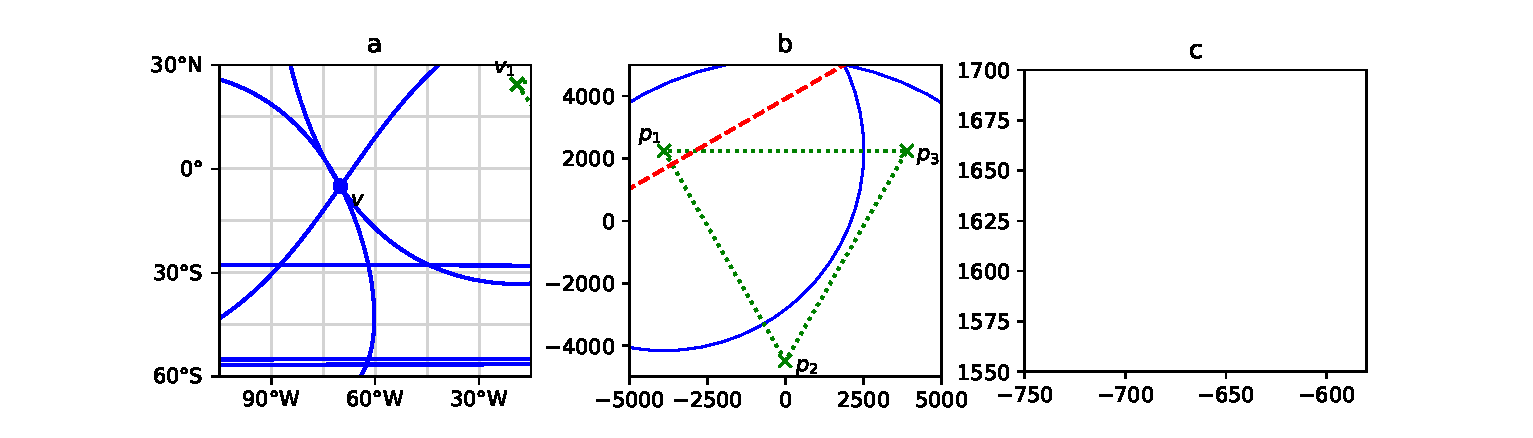
\includegraphics[width=\textwidth]{construction}
  \caption{Construction of the CTP and MTP. Plot 1a is in equirectangular
  projection. Plot 1b is the result of the CTP or MTP in the plane. Plot 1c is
  the same as plot 1b, zoomed in to the small triangle created by the three
  circles. $\mathbf p_c$ is the point projected by the CTP and $\mathbf p_m$ is
  the point projected by the MTP. Green dotted lines indicate the control
  triangles, the circles are blue solid lines,
  and the perpendiculars are red dashes.}
  \label{fig:chamberlin}
\end{figure}

Construction of the MTP starts like the CTP. If one draws a line through the two
points of intersection of each pair of circles, that line is perpendicular to
the triangle edge. These are the dashed red lines in Figure
\ref{fig:chamberlin}b and c. The three lines, one for each pair of circles,
appear to meet at a single point: this observation can be proven with a simple
triangle theorem sometimes attributed to Carnot. (\citealp{posamentier};
\citealp{wohlgemuth}) That point of intersection is denoted $\mathbf p_m$. For
most points within the control triangle $\mathbf p_m$ lies within the small
triangle, although this is not true in general and is not necessary to create a
valid map projection. (If $\mathbf v$ lies on a control triangle edge,
one pair of circles has a single point of intersection. In that case,
draw a perpendicular to the control triangle edge through that
point of intersection and continue as in the general case.)

The equations of each perpendicular line, taken together, create a linear
system. It is an overdetermined system of 3 equations in 2 variables, but since
all 3 lines meet at the same point, it has a solution. Ultimately this system
can be solved for $\mathbf p_m$ to define a forward map projection as follows.
\begin{equation}\label{eq:forward}
\mathbf p_m =
\mathbf M \begin{bmatrix*} r^2_1 & r^2_2 & r^2_3 \end{bmatrix*}^\top,
\end{equation}
\begin{equation}\label{eq:forwardm}
\mathbf M = \frac{1}{2T}
\begin{bmatrix*} y_3 - y_2 & y_1 - y_3 & y_2 - y_1 \\
x_2 - x_3 & x_3 - x_1 & x_1 - x_2 \end{bmatrix*} = \frac{1}{2T}
\begin{bmatrix*}[r] 0 & -1  \\
1 & 0 \end{bmatrix*}
\mathbf P
\begin{bmatrix*}[r] 0 & -1 & 1 \\
1 & 0 & -1 \\
-1 & 1 & 0 \end{bmatrix*},
\end{equation}
\begin{equation}\label{eq:forwardt}
T = \begin{vmatrix*} x_1 & x_2 & x_3 \\
 y_1 & y_2 & y_3 \\
 1 & 1 & 1
\end{vmatrix*}.
\end{equation}
$T$ is equal to twice the area of the Euclidean control triangle.

The matrix $\mathbf M$ has a (right) nullspace spanned by the vector
$[1, 1, 1]^\top$. This implies the MTP is not one-to-one for all possible values
of $r_i$. For example, for any values of $r_i$ such that $r_1 = r_2 = r_3$, then
$\mathbf p_m = [0, 0]^\top$. Like the CTP, the MTP projects the entire sphere to
a bounded portion of the plane: the boundary of that portion can be termed the
boundary of the projection. There is a region of overlap that is mapped into
the same area but in reverse orientation.
That region includes the antipodes of the control points. In real applications,
the overlap region of the sphere is not of interest and can be excluded.

\section{Inverse projection}
Given $\mathbf p_m$, start to invert the projection as so:
\begin{equation}\label{eq:inverse}
\begin{bmatrix*} k_1 & k_2 & k_3
\end{bmatrix*}^\top = \mathbf M^+ \mathbf p_m \,,
\end{equation}
\begin{equation}\label{eq:inversem}
\mathbf M^+ = \frac{2}{3}
\begin{bmatrix*}[r] -2x_1 + x_2 + x_3 & -2y_1 + y_2 + y_3 \\
x_1 - 2x_2 + x_3 & y_1 - 2y_2 + y_3 \\
x_1 + x_2 - 2x_3 & y_1 + y_2 - 2y_3
\end{bmatrix*} = \frac{2}{3}
\begin{bmatrix*}[r] -2 & 1 & 1 \\
1 & -2 & 1 \\
1 & 1 & -2
\end{bmatrix*}
\mathbf P^\top .
\end{equation}
$k_i = r^2_i - h$ for some value of the free parameter $h$. This is a general
solution to inverting Equation \ref{eq:forward}: $\mathbf M^+$ is the
pseudoinverse of $\mathbf M$ and vice versa. Because $\mathbf M^+$ has a left
nullspace spanned by the vector $[1, 1, 1]$, it follows that $\sum_i k_i = 0$,
and then that $h = \frac{1}{3}\sum_i r^2_i$.
These equations are not enough to determine $r_i$ and $\mathbf v$:
information about the sphere needs to be introduced.

To simplify the derivation, use $R=1$, such that distance on the surface of the
sphere has units of radians of arc. The circle of points $\mathbf v$ at
distance $r_i$ from a point $\mathbf v_i$ is simply the circle created by a
plane intersecting the sphere. Rearranging the distance function, this plane
may be specified as $\mathbf v_i \cdot \mathbf v = \cos\left(r_i\right).$
These planes combined together give a linear system. Thus,
\begin{equation}\label{eq:inversev}
  \mathbf v = \mathbf V^{-1} \begin{bmatrix*} \cos\left(r_1\right) &
  \cos\left(r_2\right) &
  \cos\left(r_3\right)
  \end{bmatrix*}^\top .
\end{equation}

For the point to lie on the unit sphere, $\|\mathbf v\| = 1$. Let $\mathbf c$
be a vector with $i$th component $\cos\left(r_i \right)$. Then,
$\mathbf c^\top \left(\mathbf V^\top \mathbf V\right )^{-1} \mathbf c = 1$.
Make the substitution
\begin{equation}\label{eq:inverser}
  r_i = \sqrt{k_i + h} \,.
\end{equation} We now have an equation with one unknown, $h$.

Some obvious bounds can be placed on $h$. In units of radians,
$0 \le r_i \le \pi$. Since this must hold for every $r_i$, it follows that
\begin{equation}
   h_{\min} = -\min_i k_i \le h \le \pi^2 - \max_i k_i = h_{\max}\,.
\end{equation}
Within these bounds, there may be at most two solutions for $h$. The solution
with smaller $h$ is the desired one, and the one with larger $h$ corresponds to
the overlap region.

Let $\mathbf A = \left(\mathbf V^\top \mathbf V\right )^{-1}$ and
\begin{equation}\label{eq:inversefh}
f(h) = \mathbf c^\top \mathbf A \mathbf c - 1 \,.
\end{equation}
The derivative of $f(h)$ is
\begin{equation}\label{eq:inversefph}
  f'(h) = -\mathbf c^\top \mathbf A \mathbf b \,,
\end{equation}
where $\mathbf b$ is a vector with $i$th component
$\mathrm{sinc}\left(\sqrt{k_i + h}\right)$.
Note that $f'(h)$ and $f(h)$ share many of the same terms, which can be
exploited for more efficient calculation. Given all the preceding, Newton's
method can be applied to solve for $h$. A suitable initial condition is
$h = h_{\min}$, which satisfies $f(h) = 0$ at the control points. This initial
condition consistently results in convergence to the lower root of $f(h)$.

The error is roughly proportional to the final value of $|f(h)|$. A stopping
condition of $|f(h)| < 10^{-4}$ results in an accuracy of 1 meter or better.
For points in or near the control triangle, this condition is met in only a
few iterations. Convergence is somewhat slower farther away from the
control triangle. At the boundary of the projection,
the lower solution and upper solution are the same and $f(h)=f'(h)=0$
so Newton's method converges at a merely linear rate. \citep{burden}

\section{Comparison}
The open-source C++ package PROJ \citep{proj} contains an implementation of the
CTP. We implemented the MTP as a patch to PROJ, to enable a fair comparison of
computation time, and to take advantage of its existing framework.

We use a set of control triangles, recorded in Table \ref{table:ctrlpts}, that
is the same as \citet[p.~90]{christensen}. These serve as a set of
test cases for comparing the CTP and MTP. The length of each side and the area
of each triangle (with the spherical approximation given earlier) is also given,
and the control triangles are sorted by area.

\begin{table}
\begin{tabular}{ p{2.5cm} | p{1.3cm} p{1.3cm} p{1.4cm} | r r r | r }
Region & \multicolumn{3}{c}{Point} &
  \multicolumn{3}{c}{Side length} &  Area \\
& 1 & 2 & 3 & 1 & 2 & 3 & \\
\hline
Africa Wall & 19°3'W, 24°25'N & 20°E, 35°S & 59°3'E, 24°25'N &
  7,783 & 7,785 & 7,783 & 32.38 \\
North \mbox{America} Wall & 150°W, 55°N & 92°30'W, 10°N & 35°W, 55°N &
  7,064 & 6,434 & 7,064 & 23.71 \\
South \mbox{America} Wall & 80°W, 9°N & 71°W, 53°S & 35°W, 6°S &
  6,161 & 5,259 & 6,947 & 17.70 \\
Europe Wall & 15°E, 72°N & 8°W, 33°N & 38°E, 33°N &
  4,254 & 4,541 & 4,541 & 9.09 \\
E South \mbox{America} & 63°33'W, 8°8'N & 58°33'W, 34°35'S & 35°13'W, 5°47'S &
  4,000 & 3,502 & 4,779 & 7.25 \\
S South \mbox{America} & 43°W, 18°S & 72°W, 18°S & 72°W, 56°S &
  4,225 & 4,874 & 3,064 & 6.77 \\
Australia & 134°E, 8°S & 110°E, 32°S & 158°E, 32°S &
  4,487 & 3,643 & 3,643 & 6.76 \\
NW South \mbox{America} & 69°W, 25°S & 55°W, 10°N & 85°W, 10°N &
  3,284 & 4,261 & 4,177 & 6.70 \\
Canada Wall & 150°W, 60°N & 97°30'W, 50°N & 45°W, 60°N &
  3,423 & 5,197 & 3,423 & 6.11 \\
Canada \mbox{Atlas} & 98°13'W, 61°39'N & 135°W, 40°N & 55°W, 40°N &
  6,560 & 3,761 & 3,449 & 5.28
\end{tabular}
\caption{Table of control triangles and their measurements. Coordinates are from
\citet{christensen}. Side $n$ is opposite point $n$. Lengths are in km,
and areas are in millions of square km.
Measurements use spherical approximation.}
\label{table:ctrlpts}
\end{table}

To measure distortion of area and angle, we use the areal scale factor $s$ and
maximum angular deformation $\omega$ as defined in equations 12--15, 27, and 28
in section 4 of \citet{snyder87}. These are implemented in the
\verb|proj_factors()| function of PROJ, which estimates the derivatives
numerically. For the projections in this text it makes sense to measure distance
distortions with regards to the distance between a given point and the control
points. Let $r_i = d(\mathbf v_i, \mathbf v)$ be the distance from
$\mathbf v_i$ to $\mathbf v$ on the sphere, as earlier, and let
$\ell_i = \|\mathbf p_i - \mathbf p\|$ be the distance from $\mathbf p_i$ to
$\mathbf p$ in the plane.
Our new measure, the total distance deviation or $D$, is the sum of
differences in the distances measured on projected and unprojected distances:
\begin{equation}
 D = \sum_i \left| r_i - \ell_i \right|.
\end{equation}

For each spherical control triangle, summary statistics for $\omega$, $D$, and
$s$ are shown in Figures \ref{fig:omegap}--\ref{fig:scalep}. Note that the
control triangles are sorted by area in these figures as well.
These statistics are measured within the spherical control triangles,
and should not be taken to summarize the entire map: in most cases,
the region of interest extends outside the triangle.
Rather, the statistics allow a quantitative comparison of the two projections.

\begin{figure}
  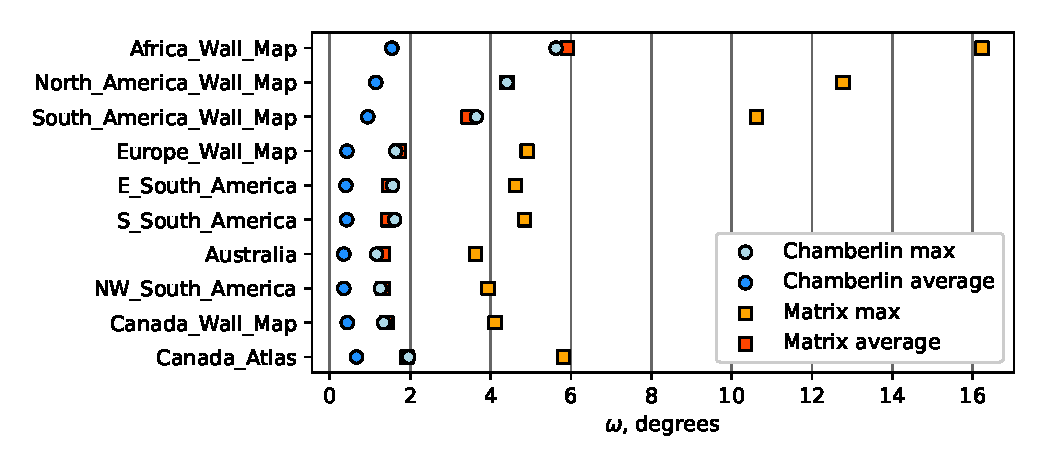
\includegraphics[width=\textwidth]{omegaplot}
  \caption{Comparison of maximum angular deformation $\omega$.}
  \label{fig:omegap}
\end{figure}

As shown in Figure \ref{fig:omegap}, the MTP consistently has a larger $\omega$
than the CTP: in fact, the maximum $\omega$ for the CTP is near the average
$\omega$ for the MTP. Maximum and average $\omega$ trend upwards with control
triangle area, although asymmetry of the control triangle has some influence
too, as can be seen in the Canada triangles. The maximum $\omega$ for the MTP
is about 3 times that for the CTP, and the average $\omega$ is about 3 to 4
times. However, for moderately-sized triangles,
the maximum $\omega$ values are small for both projections, not exceeding 6°.
Even for the large triangles -- Africa, North America, and South America Wall
Maps -- the maximum distortion is tolerable, and the average does not exceed 6°.

\begin{figure}
  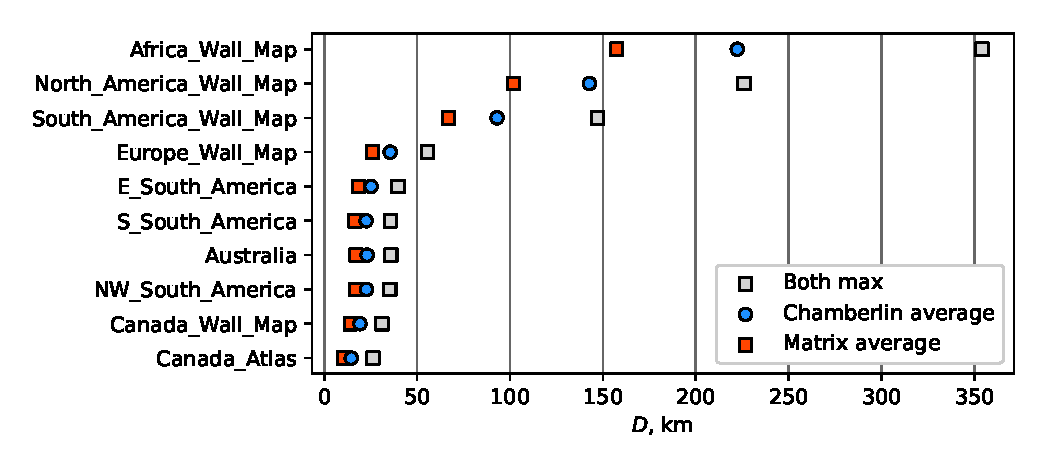
\includegraphics[width=\textwidth]{distanceplot}
  \caption{Comparison of total distance deviation $D$.}
  \label{fig:distancep}
\end{figure}

Total distance deviation $D$ in Figure \ref{fig:distancep} shows an even clearer
trend, monotonically increasing with triangle area. Both projections have the
same maximum $D$ values. The MTP has consistently lower average $D$ values than
the CTP: among these triangles, the maximum $D$ for the CTP is about
1.35 to 1.4 times the maximum $D$ for the MTP. The worst distortion,
Africa Wall Map's maximum $D$, is less than 5\% of its edge lengths, and
smaller control triangles have a maximum $D$ that is an even smaller percent.

\begin{figure}
  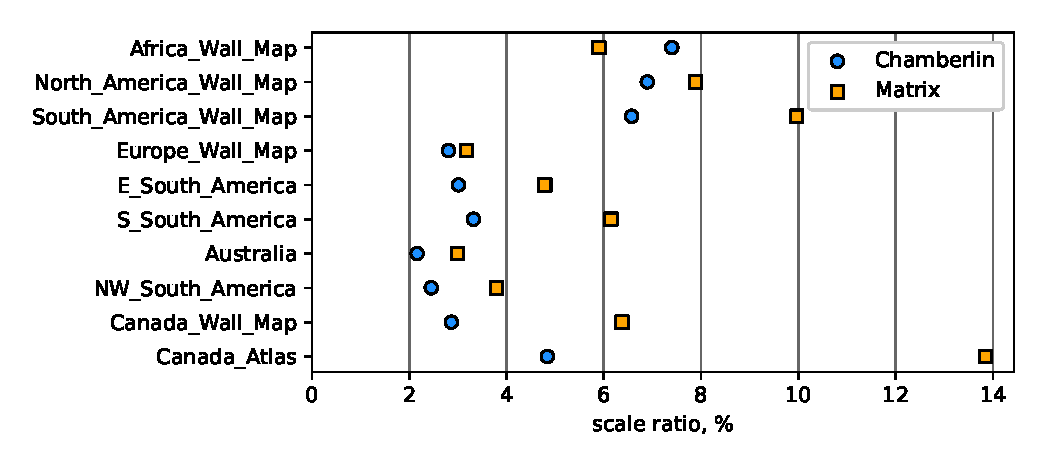
\includegraphics[width=\textwidth]{scaleplot}
  \caption{Comparison of areal scale ratio $\sigma$.}
  \label{fig:scalep}
\end{figure}

As true 1:1 scale maps are impractical, absolute values of $s$ are unimportant:
the quantity $\sigma = \frac{\max s}{\min s} - 1$ is plotted in Figure
\ref{fig:scalep} instead. The trend of $\sigma$ is less clear. A combination of
control triangle area and asymmetry influences this value. In general, this
value is higher for MTP than CTP, but not by any consistent factor,
and for the large and symmetric Africa Wall Map triangle the MTP is
actually lower than the CTP. The amount of scale distortion is small for both:
except for the very obtuse Canada Atlas triangle, all values are below 10\%.

A comparison of the two projections using the South America Wall Map control
points is in Figure \ref{fig:proj}.
The South America Wall Map control triangle is fairly
representative, being somewhat asymmetric but not too obtuse. The small part of
Central America in the upper left is somewhat shifted between the two maps, as
is the western area near Ecuador and Peru, but no features on either map are
conspicuously distorted compared to the other. Figure \ref{fig:tissot} shows
ellipses of distortion with centers on a grid at steps of 15° latitude and
longitude.
Distortion is somewhat more visible in this figure: one can see that the
MTP introduces slightly more non-conformal distortion near the control points.

\begin{figure}
  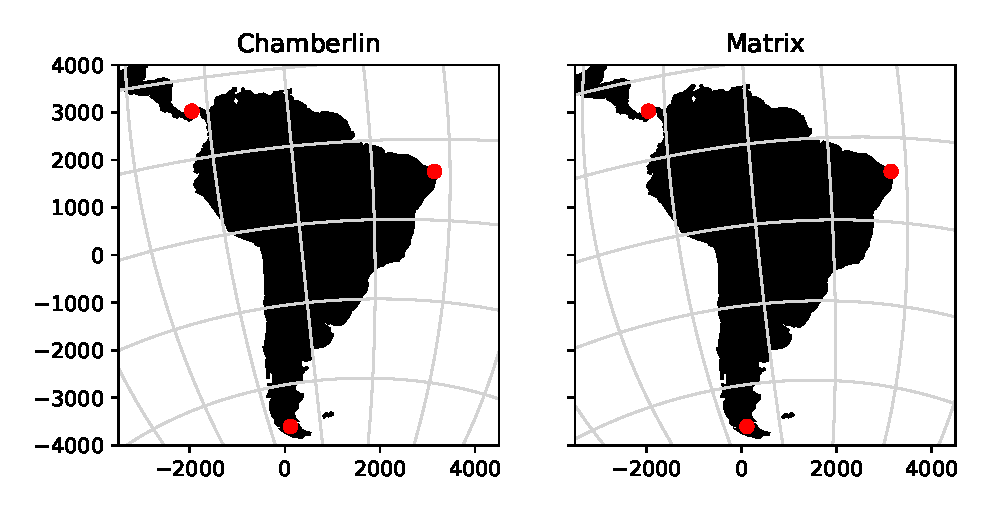
\includegraphics[width=\textwidth]{South_America_Wall_Map_zoom}
  \caption{Projection of South America and surroundings. In this and the
  following figures, red dots indicate the control points.}
  \label{fig:proj}
\end{figure}

\begin{figure}
  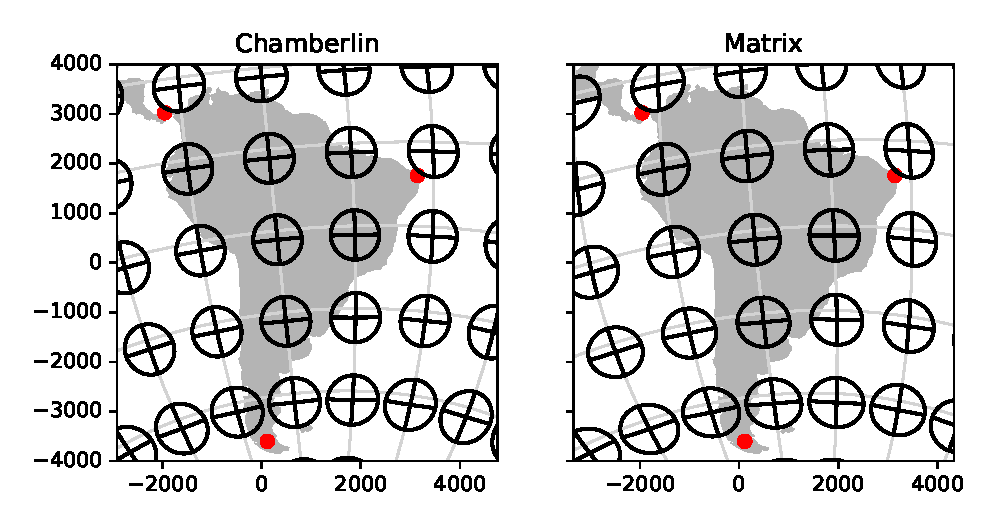
\includegraphics[width=\textwidth]{South_America_Wall_Map_tissot}
  \caption{Ellipses of distortion, on a 15° grid.}
  %FIXME cheating a little here, use a, b, theta instead?
  \label{fig:tissot}
\end{figure}

\begin{figure}
  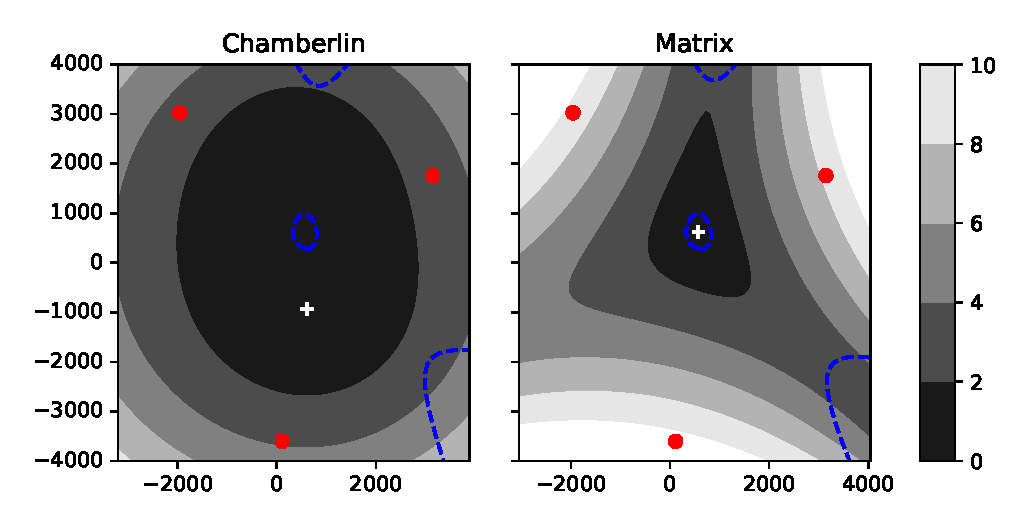
\includegraphics[width=\textwidth]{South_America_Wall_Map_omega}
  \caption{Maximum angular deformation $\omega$, in degrees. Blue dashed lines
  indicate where the two projections have equal $\omega$ values. The white
  $+$ symbol indicates where $\omega$ attains the minimum value of 0°.}
  \label{fig:angle}
\end{figure}

Contour lines of $\omega$ are shown in Figure \ref{fig:angle}. Those in the CTP
are ovals, while those for the MTP extend outward through each edge of the
control triangle. Both reach a minimum $\omega$ of 0 at a point inside the
control triangle. Highly obtuse control triangles, like Canada Atlas, may have
two local minima for $\omega$ within the control triangle. $\omega$ is higher
for MTP than CTP, except for a small region in the control triangle where both
are near 0 and some regions near the boundary of the map.

\begin{figure}
  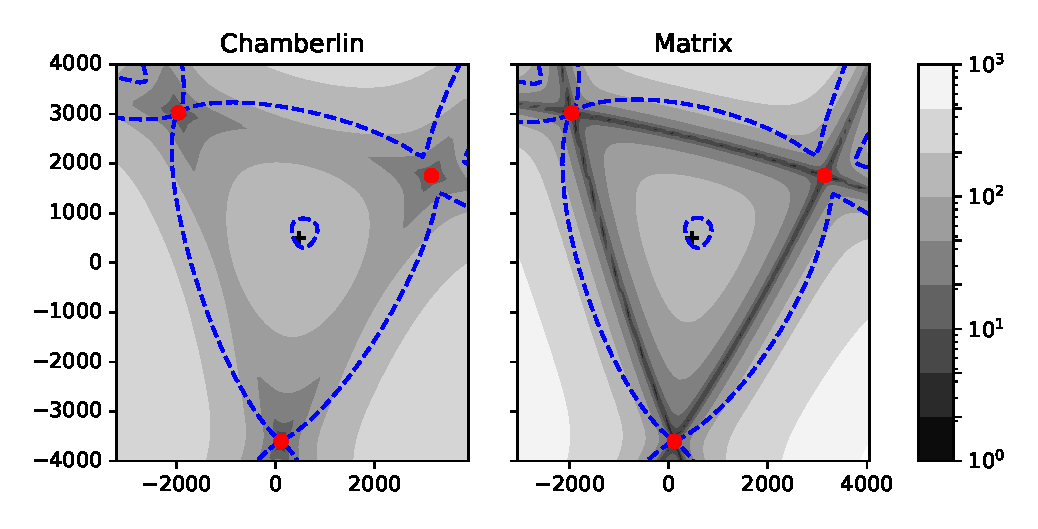
\includegraphics[width=\textwidth]{South_America_Wall_Map_distance}
  \caption{Total distance deviation $D$. Blue dashed lines indicate where the
  two projections have equal $D$ values. The black $+$ symbol indicates where
  $D$ attains a local maximum of 147 meters.}
  \label{fig:distance}
\end{figure}

Figure \ref{fig:distance} depicts contour lines of $D$ for these two
projections. Both projections have a local minimum of 0 at the control points,
which follows from the geometric construction. Both have a local maximum inside
the control triangle. $D$ for the MTP is low along the control triangle edges,
while for the CTP it is larger. $D$ is lower for MTP than CTP in a region
including the control triangle and nearly all of South America, except for a
small region near the shared maximum. It is also lower along the lines extending
out along the edges of the control triangle. $D$ does increase more rapidly for
the MTP than the CTP in the other regions outside the triangle as one moves away
from the control triangle.

\begin{figure}
  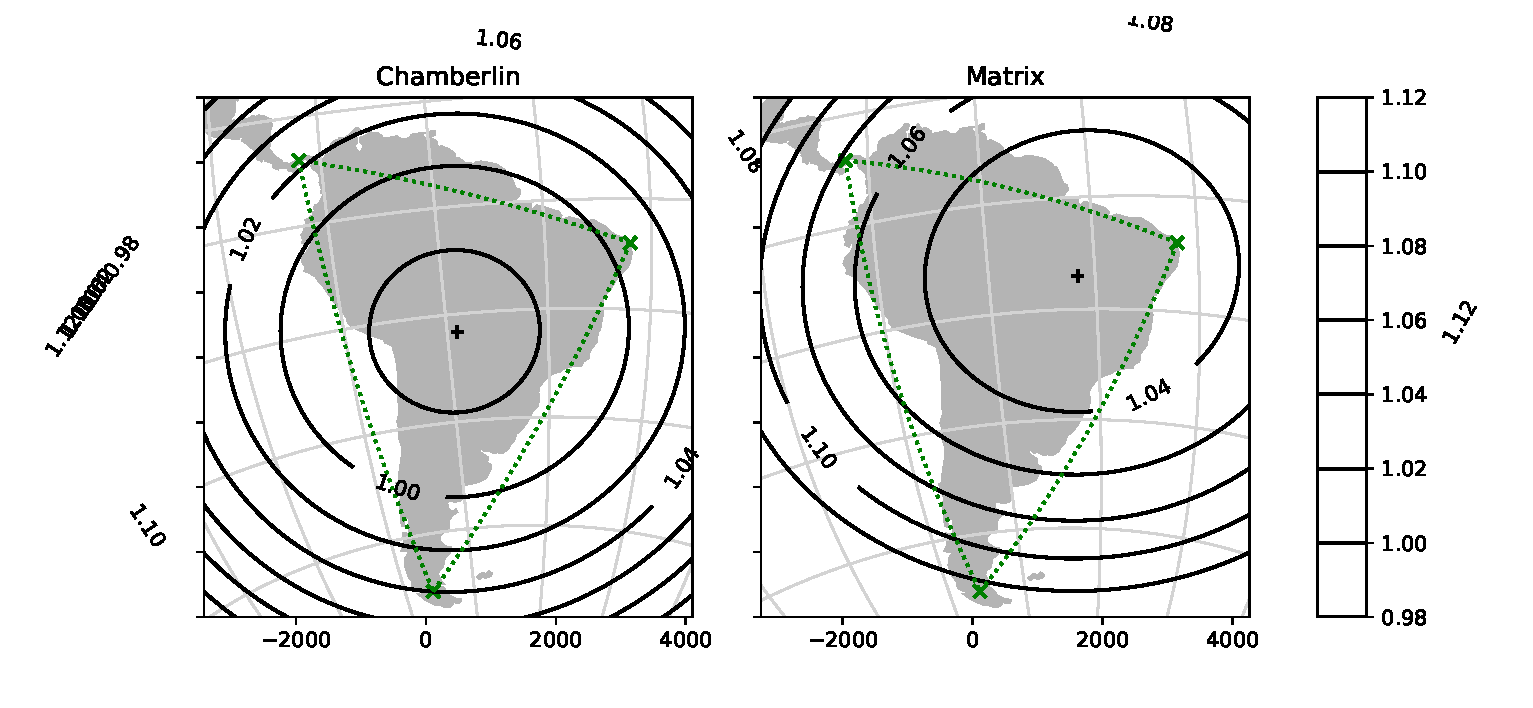
\includegraphics[width=\textwidth]{South_America_Wall_Map_scale}
  \caption{Areal scale factor $s$. The white $+$ symbol indicates where
  $s$ attains a local minimum: 0.974 for CTP and 1.022 for MTP.}
  \label{fig:scale}
\end{figure}

Contour lines of $s$ are shown in Figure \ref{fig:scale}.
The contour lines have the same elliptical structure in both projections,
centered on a point where $s$ reaches a local minimum. This point, and the
minimum value there, is different for each projection. That influences the
differences in aggregate area distortion in Figure \ref{fig:scalep}. The
spherical control triangle is projected to a slightly different shape for each
projection, which influences the unscaled values of $s$ as well.

In most practical applications the area pictured in these figures will be
sufficient, but we can state trends as both projections extend outward from the
control triangle, outside the area shown in these figures. $\omega$ increases to
180° at the projection boundary, and increases further in the overlap region,
representing the inversion there. $D$ generally increases away from the center,
but for the MTP $D$ remains low on the control triangle edges.
$s$ is bounded for the entire sphere:
it increases to a maximum and then decreases to 0 at the projection boundary.
In the overlap region, $s$ becomes negative and reaches a minimum value.

\begin{table}
\begin{tabular}{ l r r}
  Projection & Time (s) & Time minus overhead (s)\\
\hline
  CTP & 3.42 & 3.40 \\
  MTP & 1.63 & 1.62 \\
  No-op & 0.02 & 0.00
\end{tabular}
\caption{Computation time comparison.}
\label{table:time}
\end{table}

To determine computation time, the \texttt{timeit} package in Python
\citep{python} was used with the PyProj interface to PROJ. \citep{pyproj} A
data set of 64,800 points across the sphere was projected 100 times. This was
repeated 5 times for each control triangle, and the lowest total time of those 5
was recorded, as recommended by the \texttt{timeit} documentation. This was
done for the two projections and a ``no-op'' projection that returns the input
unchanged, used to estimate overhead. Only the transformation itself was timed,
not the initialization of the projection: the initialization time is negligible
compared to the time cost of running the projection repeatedly. As expected,
the timing differences between control triangles were not significant for either
projection. Table \ref{table:time} shows the minimum
runtimes across all control triangles. Accounting for overhead,
the MTP takes slightly less than half the time of the CTP.

\section{Conclusion}
We have presented a new compromise map projection, the matrix trimetric
projection (MTP), and demonstrated that it is a suitable alternative to the
Chamberlin trimetric projection (CTP). In general, the differences between the
results of the CTP and MTP are small. The MTP has the advantage if an inverse
is needed, if one wishes to reduce the distance distortion described earlier,
or if processing time is a concern. The CTP is useful for creating maps of
continents with low levels of various types of distortion,
but is uncommon in contemporary cartography:
the advantages of the MTP may open it up to new uses.

The forward formula for the MTP is given in Equations
\ref{eq:forward}--\ref{eq:forwardt}. Equation \ref{eq:forward} is a simple
product of a matrix and a vector. The vector depends on the point being
transformed. The matrix calculated by the latter two equations depends only on
the control points, so can be calculated once and reused. Measuring points
transformed per unit time, the MTP is about twice as fast as the CTP. Of
course, details of the software influence the speed comparison, but
PROJ's implementation of the CTP is itself fairly short, does not have any
obvious inefficiencies, and has changed little in more than two decades.

The inverse formula for the MTP is calculated by Equations
\ref{eq:inverse}--\ref{eq:inverser} and a single-variable Newton's method
iteration using Equations \ref{eq:inversefh} and \ref{eq:inversefph}. The
matrices in Equations \ref{eq:inversem} and \ref{eq:inversev}, as well
as matrix $\mathbf A$ in Equations \ref{eq:inversefh} and \ref{eq:inversefph},
also depend only on the control points and can be reused. The CTP,
in contrast, has no known inverse aside from the general methods used to invert
a two-variable function, which are slow and often unstable.

Figures \ref{fig:omegap}--\ref{fig:scalep} plot aggregate measures of distortion
within each of the listed control triangles. The CTP outperforms the MTP in
terms of angular distortion and (except in one case) scale distortion, but the
reverse is true for distance distortion. In most cases, the differences between
the two are small in absolute terms. For both projections, distortion tends to
be larger for a larger control triangle.
Figures \ref{fig:proj}--\ref{fig:distance} show the projections applied to
South America, demonstrating the shape of distortions across the mapped area.
Differences between the two projections in Figure \ref{fig:proj}
are difficult to notice visually.

The same control points were used for both projections in this work, but the
optimal placement of control points may be somewhat different for the
application of different projections to the same geographic feature. The
angular distortion of the MTP is lower in a region extending through the middle
of the control triangle edges, so one may wish to orient the triangle to take
advantage of that. One may also wish to avoid the area outside the triangle
where $D$ increases more rapidly for the MTP than the CTP.

The form of the MTP's forward formula suggests a possible family of projections
that are simple functions of distances to control points, such as a polynomial
function. Additionally, there may exist similar projections using measurements
other than distance, such as area.

\section{Data availability statement}
A software implementation of the MTP, as well as code used to
produce the calculations and figures in this text,
%is available on the author's Github site. \citep{trimetric}
is available at the private link https://figshare.com/s/d2f92fa8ae678cdd382c.
On acceptance this link will be replaced with an openly accessible site,
subject to Creative Commons license.

Figures in this text were created using the Python packages matplotlib
\citep{matplotlib} and GeoPandas \citep{geopandas}, and their dependencies
including PROJ \citep{proj} and PyProj \citep{pyproj} as referenced earlier.
Land mass shape data come from \citet{natearth}.

%\section{Funding}
%None.

%\section{Disclosure statement}
%The author declares no potential competing interest.

\bibliographystyle{apacite}
\bibliography{references}

\end{document}
